\documentclass[9pt,technote]{IEEEtran} 
\usepackage[numbers]{natbib}
\usepackage{graphicx}
\usepackage{subfig}

\title{TorScript: A Proposed Framework For Standardised Implementation of Countermeasures Against Attacks on Tor} 
\date{today}
\author{Jenna Finlayson~~Kurt McAlpine}

\begin{document} 
\maketitle

\begin{abstract} Tor provides anonymity by routing communications within layers
of encryption. A vulnerability in the Tor network is the indirect rate reduction
attack. This attack can reduce anonymity by monitoring client connections and
spoofing traffic on Tor exit relay. By spoofing messages to an exit relay at a
rate slower than the client was previously receiving messages, a rate reduction
can be observed. This indicates that the client is likely to be communicating
with that specific server. We propose a method to counteract this attack by
extending Tor to mask the rate of messages being received. \end{abstract}

\section{Introduction} 
The majority of surveillance that occurs today is the surveillance of data and communications on the internet \cite{diffie2008brave}. Since the 2013 leaks from Edward Snowden we now know the scale of and government power behind mass internet surveillance. It is therefore important for internet users to have a way to protect themselves from certain types of surveillance that can expose their identities and online behaviour. One solution to this is to use an anonymity network such as Tor. Tor allows anonymous communication by using layers of encryption and routing network traffic between multiple volunteer operated onion routers \cite{tor}. This aids in the concealment of the
user's physical location, identity, and usage from potential surveyors. To keep
safe from government surveillance it is important to employ countermeasures for the security vulnerabilities in Tor as they are identified.\\

New security attacks on Tor are being discovered frequently and are often published with specific ways to counteract them. Most of these proposed countermeasures come at a cost to network performance and performance of Tor and require implementations in the Tor source code directly. This requires knowledge of the Tor architecture and code base in order to implement the countermeasure, and then needs to be integrated and deployed in Tor itself. This process takes time and is not a simple process due to Tor's complexity so it therefore leaves Tor open to the identified vulnerabilities for potentially very long periods of time. \\

We propose TorScript, a framework for standardised implementation of countermeasures against attacks on Tor. [overview of stuff about how our framework works].

% Here's all the citations we have to use. 
\cite{hayesguard}\cite{gilad2012spying}\cite{sun2015raptor}\cite{biryukov2012torscan}\cite{jansen2014sniper}\cite{tor}

\section{Related Work} 
\label{sec:relatedwork}
In order to show the types of attacks that can be used to reduce the anonymity of the Tor network, we summarise papers that identify some of these types of attacks and the authors' proposed countermeasures for them. We then identify flaws in the implementation and potential deployment problems of these countermeasures. We could not find any literature about any existing standardised frameworks like the one we propose and have therefore focused on identifying different attack types that our framework can work with.\\

\subsection{Rate Reduction Attack}
To identify communicating peers in Tor, an attacker can eavesdrop on two peers they think are communicating. They can then use traffic analysis to identify patterns in the communication behaviour of both and identify similarities between them to conclude that they are indeed communicating with one another. This type of attack is difficult as it requires access to both peers to eavesdrop on the traffic behaviour. \citeauthor{gilad2012spying} have detailed a type of attack on Tor that requires only eavesdropping on the client, while carrying out an active attack on the exit relay of a Tor circuit in order to identify communicating peers.

The attack is a variant of the Idle Scan attack, however instead of trying to find open ports on a server, the authors try to determine the identity of communicating peers. To carry out the attack, three consecutive spoofed messages with invalid TCP sequence numbers are sent to the exit relay as if it came from the destination communicating peer that has a direct TCP connection to the exit relay. This causes three duplicate ACK messages to be sent from the exit relay to the destination peer which is considered to be a congestion event in TCP. As a result of the congestion event occurring, the congestion window on the destination peer is shrunk and the `sending rate' decreases. This decrease in sending rate can be seen on the origin peer as the rate of communication with the destination has been reduced. If this event is observed on the origin peer as a result of the active attack on the exit node that is communicating with the destination peer, it can be concluded that the origin and destination peer are in fact communicating.

The countermeasures that \citeauthor{gilad2012spying} have identified for this type of attack on Tor include discarding packets that do not have valid sequence numbers and also increasing the size of the congestion window so that it takes longer to cause a congestion event. Increasing the size of the congestion window on the destination peer would not be a viable robust solution as it would require all servers that could possibly be being communicated with to implement this change. It would also change the behaviour of real congestion events which could cause a loss in network performance. Similarly, by discarding out of sequence TCP packets, congestion control of actual congestion events would be modified and this would also be likely to affect network performance. 

An ideal countermeasure for this type of attack would be to modify Tor itself so that modification of destination peers is not necessary. We propose that Tor implement the ability to control the rate of sending packets so that the reduction in rate is not so observable on the origin peer.

\subsection{Guard Selection Attack}
Prior to 2015, Tor's guard selection strategy was to have each user be allocated a small set of guard nodes from which three of them would be used for extended periods. In 2015 and later, Tor's default guard selection strategy now involves users selecting one guard node from a set of nodes that are all highly available and have a high bandwidth, and using this single node for up to nine months. Both of these selection strategies have security vulnerabilities that allow attackers to identify communicating peers as identified by \citeauthor{hayesguard}.

The attacks identified that involve these guard selection strategies include:
\begin{itemize}
\item \textbf{Direct Observation:} With one corrupt guard node and a small selection of corrupt exit relays, at least one circuit can be identified for a particular user.
\item \textbf{Guard Fingerprinting:} Identifying the set of guards used by a user, which is likely to be unique to that user and hence act as a fingerprint.
\item \textbf{Statistical Disclosure Attacks:} In the case that a given guard set is only used by a small number of users, it is possible to discover long term identifiers through analysing their patterns of actions.
\end{itemize}

\citeauthor{hayesguard} have proposed a new method for guard selection involving the use of ``Guard Sets''. Guard sets are sets of relays that are used by many users and each set provides a certain amount of bandwidth. This approach counteracts the three attack types outlined above. Having no rotation of guard nodes for users means that fewer clients are exposed to malicious nodes which counteracts Direct Observation attacks. Because each guard set is used by many users, Guard Fingerprinting cannot be used to uniquely identify users. Finally, Statistical Disclosure Attacks also cannot be used on guard sets due to there being large and equal sets of users for each guard set.

\citeauthor{hayesguard} have designed an algorithm to automatically assign guards and users to guard sets. This means that there is little left to counteracting these attacks other than writing the implementation into the Tor application. This, as explained earlier, is not a trivial problem due to the complexity of the Tor code base. Once it is implemented, it would take time to be approved and accepted into the code base as well then getting deployed.

\subsection{Tor Scanning Attacks}
\citeauthor{biryukov2012torscan} propose five different scanning attacks on Tor to reduce anonymity. The first attack exposes existing TLS connections a particular Tor relay has with other relays by scanning the Tor relay in question. As Tor uses canonical connections, i.e. reuses already open connections when another connection is requested, it is possible to identify existing connections between relays. When sending a \texttt{RELAY EXTEND} cell, the destination fingerprint and IP must be specified. In the case that a connection already exists, the IP is ignored and the existing connection is used. A \texttt{RELAY EXTENDED} cell is then returned back to the origin relay to confirm. If the two relays do not have an existing connection, a new one is attempted to be created using the provided IP address. If the IP address specifies an unreachable port, the connection is refused and a \texttt{DESTROY} cell is returned. Using this information, attackers can send \texttt{RELAY EXTEND} cells to specific Tor relays, giving the fingerprint of the Tor relay in question and an unreachable port. Based on the type of cell that is returned, it can be determined whether the two relays had an existing connection open or not. The authors mention that a possible way to counteract this attack is to use both the fingerprint and IP address to identify a connection rather than just a fingerprint. However, this countermeasure opens Tor to denial of service attacks by exhausting the resources on a relay.\\

The second attack identified by \citeauthor{biryukov2012torscan} uses the same tactics as above but uses timing information to detect whether a new connection had to be made, and this time sends a reachable port to connect to. In the case that the two relays did not have an existing connection, a TLS connection is set up which takes a significant and observable amount of time to do. In the case that there is an existing connection, no new TLS connection needs to be established and so the time to receive a confirmation from the destination relay is significantly less. The countermeasures suggested by the authors for this attack include the same one as for the previous attack, but also to provide enough noise that this attack would not be reliable.\\

The third attack identified by \citeauthor{biryukov2012torscan} is the One-Hop Attack. This attack requires the attacker to be in control of one or more fast exit nodes in the Tor network and therefore see a large amount of Tor traffic pass through them. As the attacker is in control of an exit node, he/she can see information such as cookies that come from the sender. Using the methods described in the previous two attacks, the attacker scans the middle relay for connections with other nodes. One of the nodes in the resulting set of connected nodes will contain the guard node. This therefore identifies the complete circuit, identifying the sender and relating that to the data it sees pass through the exit node. This attack is aimed at long-lived connections in Tor so that the scanning can be continued over hours and days to identify a smaller and smaller set of possible guard nodes.\\

The fourth attack identified was the Two-Hop Attack. This attack is much like the One-Hop Attack but does not require the attacker to have control of an exit node. The attack can be carried out by a server or an attacker close to the server by first using the scanning technique to determine potential middle nodes (by scanning the exit node), and then scanning these potential middle nodes for connections to potential guard nodes, i.e. requiring ``two hops''.\\

The fifth attack identified was the Differential Scan Attack. This attack presumes the attacker again has control over one or more fast exit nodes and makes use of recurrent connections (e.g. refreshing of a news website to update feed). The attacker scans the middle node to determine a set of possible guard nodes as in the One-Hop Attack. Once this set is determined, the attacker sends \texttt{DESTROY} cells to each node, resulting in circuit termination. After three minutes, the scan is repeated and the difference between the two sets is observed. After repeating this multiple times, the users three guard nodes can be identified.

By employing the countermeasures described in the first two attacks, the One-Hop Attack, Two-Hop Attack, and the Differential Scan Attack would not be possible.\\

\subsection{Sniper Attack}
The sniper attack outlined by \citeauthor{jansen2014sniper} describes a denial
of service attack that can be targeted to any Tor node. The attack is relatively cheap as the attacker only needs 92 KiB/s upstream to start consuming memory at 2187 KiB/s. The way the attack works is by starting a large download over the Tor network, and then stopping the reading from the entry relay. The attacker then maliciously sends \texttt{SENDME} requests to the exit relay, forcing the entry relay to queue up cells to send to the client. The Linux OOM killer will kill the tor process when the machine runs out of memory, disabling that node in the Tor network.

The countermeasure suggested by \citeauthor{jansen2014sniper} for this attack involves monitoring the amount of free memory a machine that is used as a Tor node has, and selectively killing circuits when the amount of free memory is below a certain threshold. This would require the modification of the Tor source code.

\subsection{Routing Attacks}
A suite of attacks described by \citeauthor{sun2015raptor} includes attacks that can be performed by Autonomous System (AS) adversaries. Here we describe the high level details of each of the attacks described in the paper.

\subsubsection{Asymmetric Traffic Analysis Attack}
This attack extends the well known ``end-to-end timing analysis attack'' whereby communication is observed between the client and the entry relay as well as the traffic between the exit relay and the destination. Using this information the attacker can correlate the timing data to determine whether the client is communicating with the destination. In the conventional attack the adversary needs to monitor both the forward traffic from the client to the entry relay and from the exit relay to the destination relay. Additionally, the backward traffic from the entry relay to the client, and from the destination to the exit relay needs to be monitored. This is difficult as the routes for the forward and backward traffic are often not the same. 

\citeauthor{sun2015raptor} describes the asymmetric traffic analysis attack as only needing to observe traffic in one of the directions to correlate the data and determine if the client is communicating with the destination. This attack increases the ability of AS-level adversaries to deanonymise Tor users by increasing the amount of ASs that can correlate the data.\\

\begin{figure}[h!]
\centering
\subfloat{{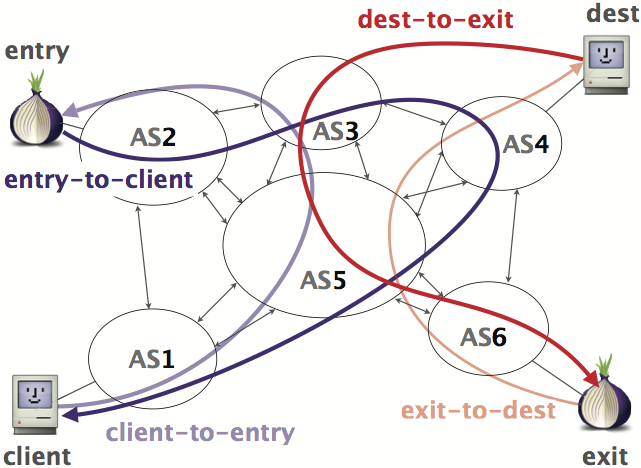
\includegraphics[width=0.2\textwidth]{images/routing1.png}}}
~~
\subfloat{{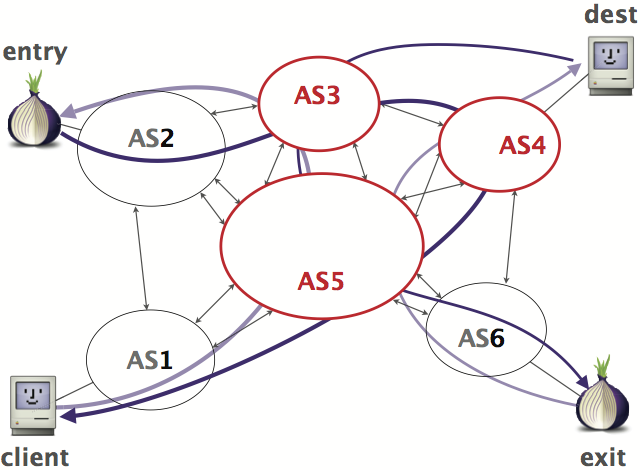
\includegraphics[width=0.2\textwidth]{images/routing2.png}}}
\caption{AS-level surveillance \cite{sun2015raptor}}
\label{fig:as-routing}
\end{figure}

In figure \ref{fig:as-routing} it is possible to see that if you need to capture traffic in both directions, only AS5 can perform the attack, but if only one direction is needed, AS3, AS4, and AS5 can perform the attack.\\

\subsubsection{BGP Churn}
The internet paths between clients and Tor relays change over time due to
physical changes in the network topology. This is known as the Border Gateway Protocol (BGP) Churn. This can be caused by system failures, system recoveries, the introduction of new routers and links, and changes to AS-level routing policies. These changes can increase the ability of ASs to observe Tor traffic. For example, in figure \ref{fig:as-churn} it can be seen that only AS5 can compromise anonymity, but when the link between AS5 and AS4 is destroyed, AS5 and AS3 can compromise anonymity.\\

\begin{figure}[h!]
\centering
\subfloat{{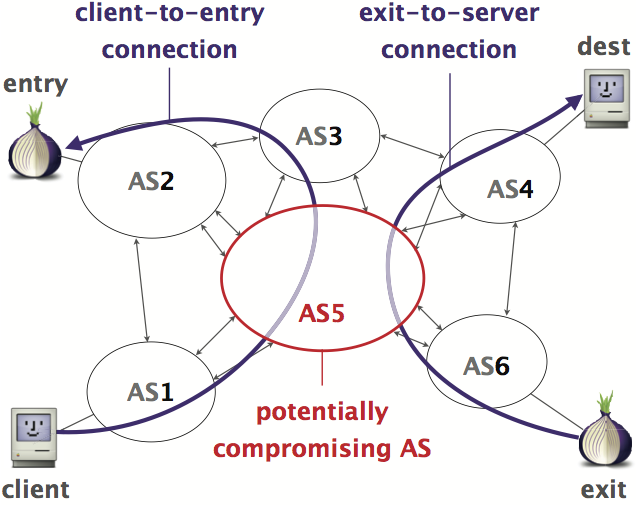
\includegraphics[width=0.2\textwidth]{images/churn1.png}}}
~~
\subfloat{{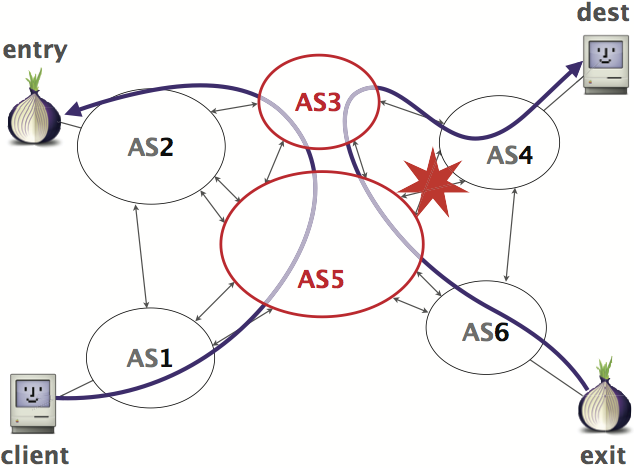
\includegraphics[width=0.2\textwidth]{images/churn2.png}}}
\caption{Network topology changes \cite{sun2015raptor}}
\label{fig:as-churn}
\end{figure}

\subsubsection{BGP Hijack}
The previous two attacks that were described were passive, but it is also possible for ASs to launch active attacks. It is possible for an AS to deviate from the default routing behaviour by manipulating inter-domain routing by communicating fake BGP control messages. An AS can hijack an IP prefix by announcing the prefix as its own. This attack will cause some small percentage of the internet traffic that was destined to the prefix to be collected by the malicious AS. This allows ASs to increase their chance of observing traffic between clients and entry relays, and exit relays and destinations. However, the disadvantage of this attack is that the traffic is silently dropped without telling the source that the data has not reached the recipient resulting in the connection being dropped.\\

\subsubsection{BGP Interception}
The authors describe an attack called BGP Interception which allows an AS to be
an intermediate between the entry relay and the client as well as between the
exit relay and the destination. The advantage of BGP Interception is that the
connection is not dropped allowing the connection to stay alive, unlike the BGP
Hijack. It is shown that 90\% of Tor relays are vulnerable to interception
attacks. This attack increases the ability of an AS to perform the Asymmetric
Traffic Analysis Attack.\\ 

\subsubsection{Countermeasures}
\begin{itemize}
\item \textbf{AS-Aware Path Selection:} Selecting the Tor relays that will be in
	the path allows us to minimise the potential for AS-level traffic
	analysis. The Tor network can monitor the path dynamics between entry
	relays and clients as well as between exit relays and destinations. This
	data can be distributed to all Tor clients and then Tor clients can use
	this information to make relay path selections. Tor clients would select
	relays such that the same AS is not in the first and last segment of the IP
	address.
\item \textbf{Advertising /24 Tor prefixes:} More than 90\% of Tor relays use a
	prefix length shorter than /24. This makes them vulnerable to the BGP
	hijack or interception attacks since ASs usually filter route
	advertisements with a prefix longer than /24. To counteract this, the prefix length used should be longer than /24.
\item \textbf{Favouring Closer Guard Relays:} Even if a Tor relay advertises a
	/24 prefix, it is still possible for an adversary to launch a specific
	prefix hijack or interception attack. If this is the case, the impact is
	limited to localised attacker's ASs since the route is not globally
	propagated. Tor clients should choose their guard relays with a shorter
	AS-level path between them. This reduces the risk of a specific prefix
	attack as well as the risk of asymmetric traffic analysis and BGP churn.
\end{itemize}

\section{TorScript: A Proposed Plugin Architecture for Tor}
Currently the Tor project is a significantly large application written in C,
with around 216000 lines of code. The size of the project and the lack of an
extensible API provides a high barrier of entry to making modifications to the
project. We want to make it easier for developers and researchers to extend Tor, especially to implement countermeasures that are often presented in academia. If it was easier to modify Tor, the time it takes for security issues to be resolved would be significantly reduced from when they are discovered.\\

We propose exposing the internals of Tor with a scripting language such as
Python. This will allow developers and researchers to write small amounts of
code to extend Tor to fix security issues. The choice of Python is to reduce the complexity of making a modification to Tor as C is an unforgiving language and requires a high degree of experience to write robust and secure code.

\subsection{Exposing Important Sections of Tor}
Several areas of the Tor internals will need to be exposed by the Python plugin
architecture. In this section we describe the main areas of interest in the Tor
code that will need to be exposed to implement Python script plugins to prevent
the vulnerabilities described in section \ref{sec:relatedwork}.\\

\subsubsection{Rate Reduction Attack}
To implement our proposed countermeasure for the rate reduction attack described in \cite{gilad2012spying} a plugin for making the rate of message sending consistent would need to be written. This would not require any interacting with Tor but the plugin itself can automate the sending.

\subsubsection{Guard Selection Attack}
This would require a plugin for the path selection hook that changes which nodes are used for the entry nodes. This would require exposure to the client tor code for selecting paths.

\subsubsection{Tor Scanning Attacks}
Use the connection hook to create a new connection and identify connections by both parameters, not just one. Also just send noise like in the rate reduction attack. Needs access to the channel_tls_handle_incoming in the channeltls.h file.

\subsubsection{Sniper Attack}
For the countermeasure suggested by \citeauthor{jansen2014sniper} for Sniper Attacks, control over circuits in needed as well as access to the amount of free memory. Free memory can be exposed from the operating system using the standard Python library \texttt{os} and circuits can
be closed through the method \texttt{circuit\_mark\_for\_close} in the
\texttt{circuitlist.h} header. These can easily be exposed with a Python
binding.\\

\subsubsection{Routing Attacks}
The countermeasures suggested for Routing Attacks by \citeauthor{sun2015raptor} require the following:
\begin{itemize}
\item Collecting data about the location of Autonomous Systems.
\item Distributing this data to clients.
\item Making relay path selection based on this data.
\item Changing the prefix length.
\item Favouring entry relays with the shortest AS-level path.
\end{itemize}

This will require exposing the path selection controls for the client and exposing the prefix length controls on the Tor server.

\subsection{Architecture}
Several different hooks will be made available to a plugin developer. Depending on
the hooks the developer wants to make use of, the developer will add a script to
the corresponding directory. The hook directories are proposed as follows:
\begin{itemize}
\item \texttt{startup/} All the scripts in this directory are run before Tor starts
	running so that certain parameters may be set.
\item \texttt{async/} For scripts that will be running continuously while Tor is
	running. This allows the plugin developers to write plugins that change
	Tors behaviour on the fly.
\item \texttt{path\_selection/} This allows for modification of the path
	selection algorithm used by Tor clients.
\end{itemize}
These hooks can be added to Tor simply by making modification to
\texttt{or/main.c} in the Tor codebase. The startup and async hooks can be added
to the top of the \texttt{main} function.


\section{Conclusion}
By exposing the internals of Tor through a scripting language it allows a wider
range of contributors to make modifications to Tor. If we expose it using a
popular language such as Python it reduces the skill level required to make
changes. It also allows for a variety of plugins to be produced for Tor, of
which Tor operators may choose which plugins they would want to install based
on their needs. It also allows researchers to actually implement the solutions
they suggest in their papers allowing them to robustly verify their results.

\bibliographystyle{IEEEtranN}
\bibliography{references}

\end{document}
